\documentclass[../../time_series_notes.tex]{subfiles}
\begin{document}
%%%%%%%%%%%%%%%%%%%%%%%%%%%%%%
\section{ARIMA(p,d,q) Process}
A process $X$ is said to be ARIMA(p,d,q) with AR of order $p$ and MA of order $q$ if the process $\nabla^{d}X_{t} = (1-B)^{d}X_{t}$ is ARMA(p,q).\newline

Thus, Autoregressive Integrated Moving Average process is an extension of ARMA to non stationary data. The difference operator simply allows removal of any trend that may exist in the data. Mathematically, the equation is similar to ARMA
\begin{align*}
    \phi(B)X_{t} &= \beta(B)W_{t} \quad &\mbox{ARMA(p,q)}\\
    \phi(B)\nabla^{d}X_{t} &= \beta(B)W_{t} \quad &\mbox{ARIMA(p,d,q)}\\
\end{align*}

\begin{figure}[h]
    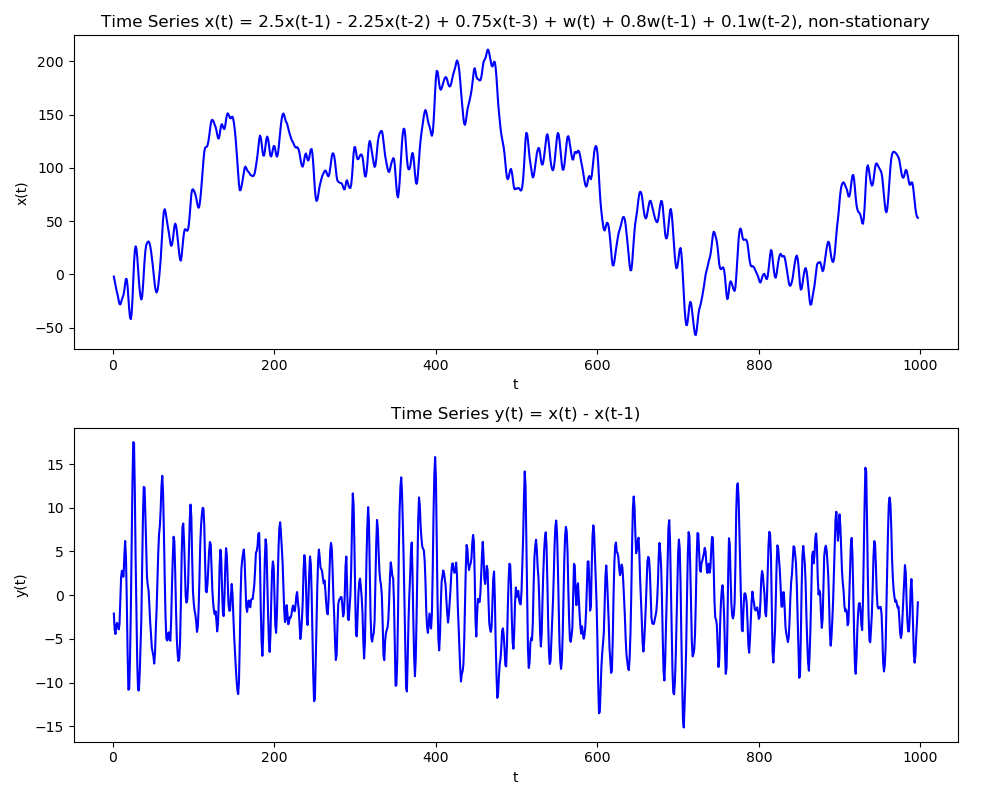
\includegraphics[scale=0.5]{arima_1}
    \centering
    \caption {Top figure shows an ARIMA(2,1,2) time series, which is clearly non stationary as the covariance varies wildly. Bottom plot shows the differenced series which is stationary. Figures plot using arima\_simulation.py}
    \label{fig:arima_1} %\ref{fig:arima_1}
\end{figure}

Usually, differencing of 1 or 2 will be enough in practical situations. If we directly observe a trend in the time series, we will know to use ARIMA instead of ARMA. Furthermore, ACF can indicate the need for differencing as it will have a very slow decay.\newline

The following information comes in handy when deciding the parameters from ACF and PACF plots
\begin{itemize}
    \item The data may follow ARIMA(p,d,0) if the plots of differenced data show
    \begin{itemize}
        \item ACF is exponentially decaying or sinusoidal
        \item PACF has a significant spike at lag $p$, but none beyond that
    \end{itemize}
    \item The data may follow ARIMA(0,d,q) if the plots of differenced data show
    \begin{itemize}
        \item ACF has a significant spike at lag $q$, but none beyond that
        \item PACF is exponentially decaying or sinusoidal
    \end{itemize}
\end{itemize}

We can now laydown the following steps to follow for determining the orders of an ARIMA process
\begin{itemize}\label{arima_model}
    \item Plot the series to understand any trend in it. This will suggest differencing. We can to repeated differencing until the series begins to look stationary.
    \item If the variance is also changing with time, a transformation might be needed. Common transformation will be log. Usual procedure then becomes to first take the log, and then do the differencing.
    \item After the transformations, ACF can suggest the order $p$ of AR process. Usually, we try out a couple of values near the estimated $p$.
    \item Similarly, PACF can tell the order $q$ of MA process. Again, different values can be tried.
    \item To determine the best combination of ($p$, $d$, $q$), we will compare the AIC values of different models. The simplest model with lowest AIC must be picked. AIC is used as it takes into account the number of parameters as well.
    \item Residuals can be estimated and must be checked to ensure that they are normal with 0 mean. This can be done through the Q-Q plot. This plot compares the percentile wise distribution of the standardized residuals (residuals/deviation of residuals) with the theoretical distribution of a standard normal. In an ideal scenario this should be a straight line.
    \item We should also check the assumption that the residuals at different lags are not correlated. This can be done by plotting the ACF of residuals.
    \item Ljung-Box Test can help check the hypothesis that the values of different correlation coefficients are indeed non zero. This can be done by plotting the $p-value$ of the statistic as a function of lags.
\end{itemize}

\subsection{Ljung–Box Hypothesis Test}
This is a useful hypothesis testing method that can help check if at least one of the autocorrelation coefficients is non zero. 
\begin{align*}
    &H_{0}: \text{the data points are independent; no correlations exists at given lag}\\
    &H_{1}: \text{at least one correlation between different lags is non zero}
\end{align*}
The test statistic is
\begin{align*}
    Q = n(n+2) \sum_{k=1}^{h}\frac{\hat{\rho}_{k}}{n-k}
\end{align*}
where $n$ is the number of samples, $h$ is the lags for which the hypothesis is being tested, and $\hat{\rho}_{k}$ is the autocorrelation coefficient at lag $k$. Under the null hypothesis that all coefficients are 0 and exhibit no correlation,
\begin{align*}
    Q \sim \chi_{h}^{2}
\end{align*}

Hence, for $1-\alpha$ confidence interval dictates that
\begin{align*}
    \text{Accept $H_{0}$ if } \quad Q < \chi_{1-\alpha, h}^{2}
\end{align*}
or, the test statistic is sufficiently less than the $1-\alpha$ $\chi_{h}^{2}$ value.



\subsection{SARMA Process}
A seasonal ARMA process operates on the seasonal terms of the original time series. Mathematically,
\begin{align*}
    \Phi(B^{s})X_{t} &= \mathcal{B}(B)W_{t}\\
    X_{t} &= \Phi_{1}X_{t-s} + \cdots \Phi_{p}X_{t-sp} + W_{t} + \mathcal{B}_{1}W_{t-s} + \cdots + \mathcal{B}_{q}W_{t-sq}
\end{align*}

So a series with an annual period might become
\begin{align*}
    (1 - \Phi_{1}B^{12} - \Phi_{2}B^{24})X_{t} &= (1 + \mathcal{B}_{1}B^{12})W_{t}\\
    X_{t} &= \Phi_{1}X_{t-12} + \Phi_{2}X_{t-24} + W_{t} + \mathcal{B}_{1}W_{t-12}
\end{align*}

The conditions for stationarity and invertibility still remain the same, but instead of polynomials of $z$, we now have polynomials of $z^{s}$.

\begin{figure}[h]
    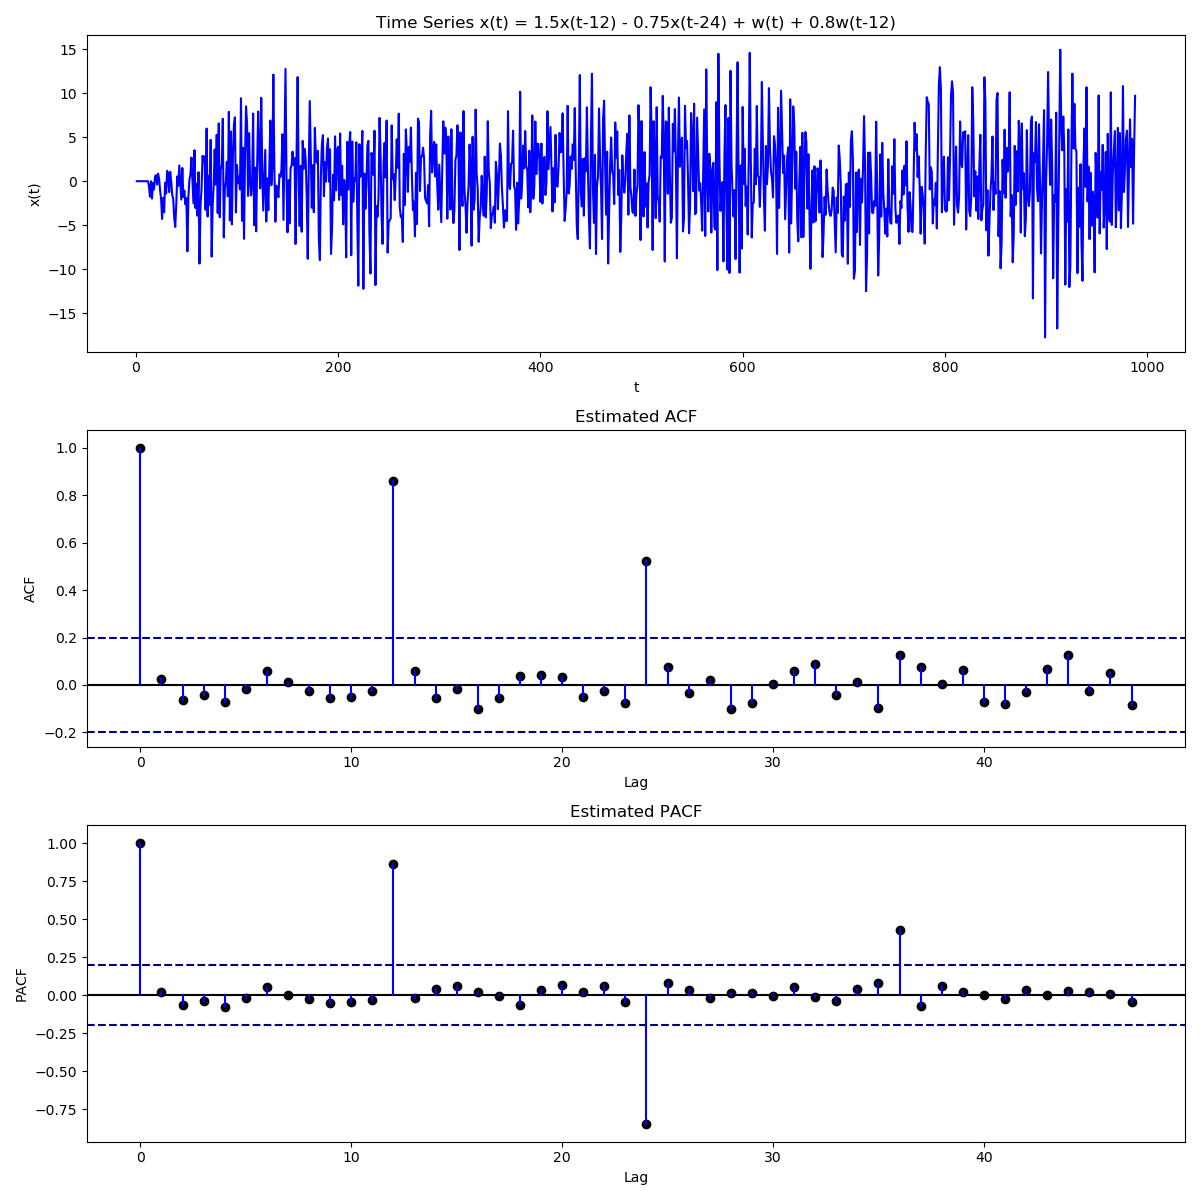
\includegraphics[scale=0.4]{sarma_1}
    \centering
    \caption {Top figure shows a time series, with the sample ACF and sample PACFs shown by middle and bottom figures respectively. We can always ignore the peak at lag 0. Both ACF and PACF have peaks at lags 12, 24. This almost goes hand in hand with the SARMA(2,1)12 time series, the ACF peak at 24 suggests a second order MA term as well. The dotted lines are noise lines and in practice, we ignore any peak below these. Figures plot using sarma\_simulation.py}
    \label{fig:sarma_1} %\ref{fig:sarma_1}
\end{figure}

We can even have both seasonal and non seasonal components together
\begin{align*}
    \Phi(B^{s})\phi(B)X_{t} &= \mathcal{B}(B)\beta(B)W_{t}\\
    (1 - \Phi_{1}B^{12} - \Phi_{2}B^{24})(1 - \phi_{1}B)X_{t} &= (1 + \mathcal{B}_{1}B^{12})(1 + \beta_{1}B)W_{t}
\end{align*}
For such a series, we expect to not only see seasonal peaks in the ACF and PACF plots, but also peaks near these seasonal peaks.

\begin{figure}[h]
    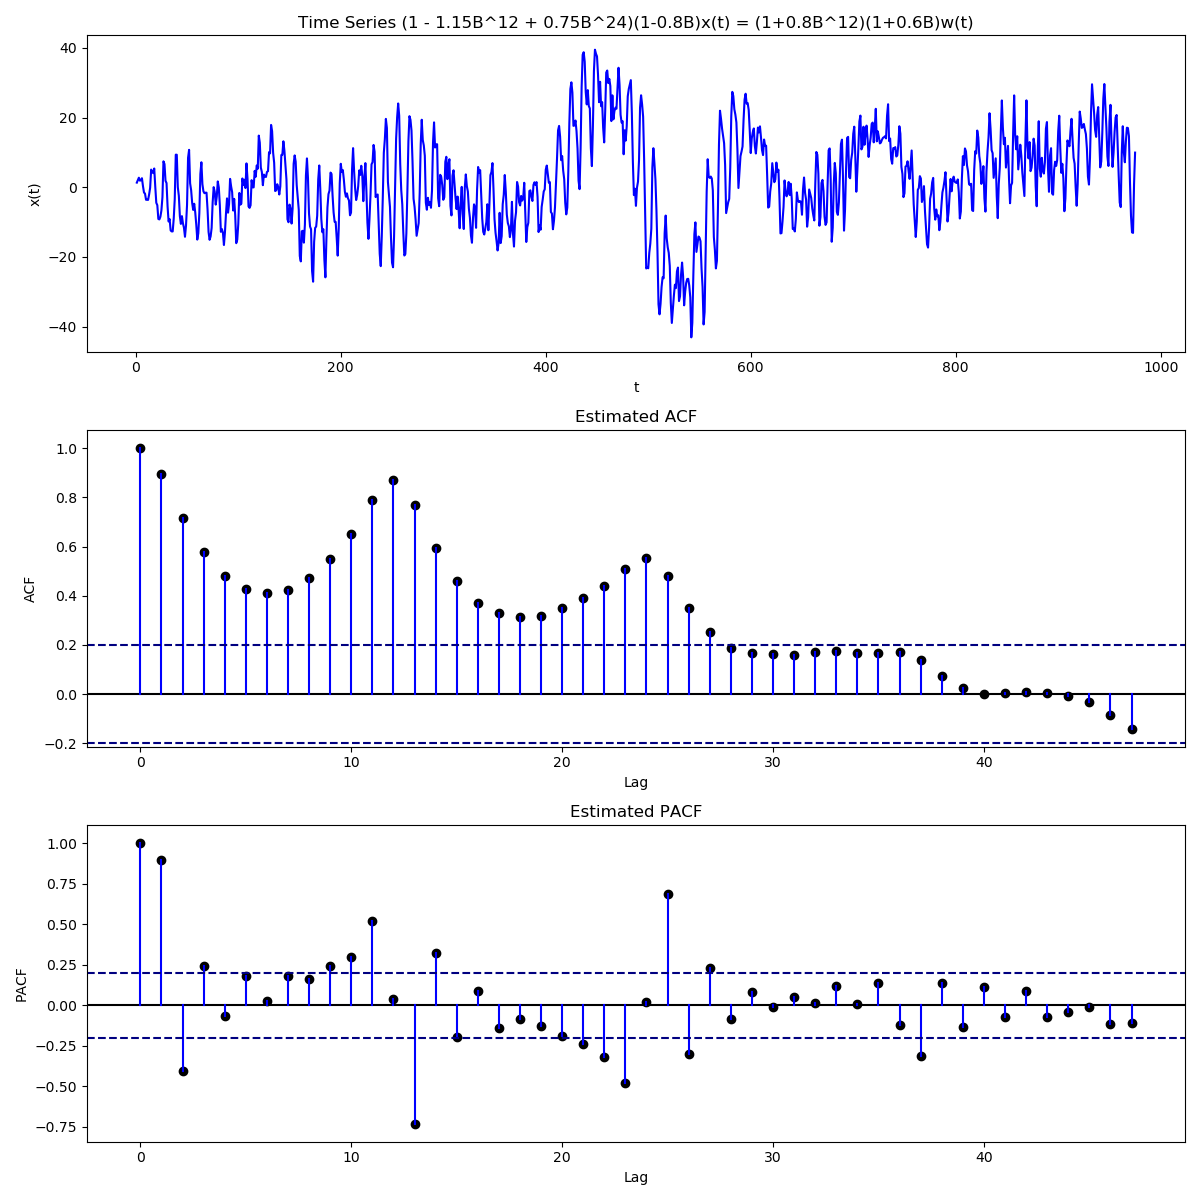
\includegraphics[scale=0.4]{sarma_2}
    \centering
    \caption {Top figure shows a time series, with the sample ACF and sample PACFs shown by middle and bottom figures respectively. We can always ignore the peak at lag 0. The dotted lines are noise lines and in practice, we ignore any peak below these. Figures plot using sarma\_simulation\_1.py}
    \label{fig:sarma_2} %\ref{fig:sarma_2}
\end{figure}


\subsection{SARIMA Process}
Building on SARMA, SARIMA(p,d,q,P,D,Q)s process is defined as
\begin{align*}
    \Phi(B^{s})\phi(B)(1-B^{s})^{D}(1-B)^{d}X_{t} &= \mathcal{B}(B^{s})\beta(B)W_{t}\\
    \Phi(B^{s}) &= 1 - \Phi_{1}B^{s} -\Phi_{2}B^{2s} - \cdots - \Phi_{P}B^{Ps}\\
    \phi(B) &= 1 - \phi_{1}B - \phi_{2}B^{2} - \cdots - \phi_{p}B^{p}\\
    \mathcal{B}(B^{s}) &= 1 + \mathcal{B}_{1}B^{s} + \mathcal{B}_{2}B^{2s} + \cdots + \mathcal{B}_{Q}B^{Qs}\\
    \beta(B) &= 1 + \beta_{1}B + \beta_{2}B^{2} + \cdots + \beta_{q}B^{q}
\end{align*}
The various parameters of SARIMA are defined as follows
\begin{itemize}
    \item $p$: non-seasonal AR order
    \item $d$: differencing of the non-seasonal part
    \item $q$: non-seasonal MA order
    \item $s$: seasonality of series
    \item $P$: seasonal AR order
    \item $D$: differencing of the seasonal term (i.e., $\nabla^{D}B^{s}$)
    \item $Q$: seasonal MA order
\end{itemize}

By bringing seasonal terms in ARIMA, we extend the modelling steps defined in \ref{arima_model}
\begin{itemize}
    \item The differencing can now be also done at the seasonal level; the order of differencing does not matter, i.e., seasonal differencing can be done before or after the non-seasonal differencing, this comes from the formula $(1-\mathcal{B}^{s})(1-\beta(B))$.
    \item Transformations like log can still be applied before differencing to limit variance/remove trends
    \item Adjacent peaks in ACF give the MA order
    \item Peaks at seasonal lags in ACF give the seasonal MA order
    \item Adjacent peaks in PACF give the AR order
    \item Peaks at seasonal lags in PACF give the seasonal AR order
    \item Since so many terms are involved, a rule of thumb serves well to reduce model complexity
    \begin{align*}
        p+d+q+P+D+Q \leq 6
    \end{align*}
\end{itemize}
\end{document}